% Options for packages loaded elsewhere
\PassOptionsToPackage{unicode}{hyperref}
\PassOptionsToPackage{hyphens}{url}
%
\documentclass[
  12pt,
]{article}
\usepackage{lmodern}
\usepackage{setspace}
\usepackage{amssymb,amsmath}
\usepackage{ifxetex,ifluatex}
\ifnum 0\ifxetex 1\fi\ifluatex 1\fi=0 % if pdftex
  \usepackage[T1]{fontenc}
  \usepackage[utf8]{inputenc}
  \usepackage{textcomp} % provide euro and other symbols
\else % if luatex or xetex
  \usepackage{unicode-math}
  \defaultfontfeatures{Scale=MatchLowercase}
  \defaultfontfeatures[\rmfamily]{Ligatures=TeX,Scale=1}
\fi
% Use upquote if available, for straight quotes in verbatim environments
\IfFileExists{upquote.sty}{\usepackage{upquote}}{}
\IfFileExists{microtype.sty}{% use microtype if available
  \usepackage[]{microtype}
  \UseMicrotypeSet[protrusion]{basicmath} % disable protrusion for tt fonts
}{}
\makeatletter
\@ifundefined{KOMAClassName}{% if non-KOMA class
  \IfFileExists{parskip.sty}{%
    \usepackage{parskip}
  }{% else
    \setlength{\parindent}{0pt}
    \setlength{\parskip}{6pt plus 2pt minus 1pt}}
}{% if KOMA class
  \KOMAoptions{parskip=half}}
\makeatother
\usepackage{xcolor}
\IfFileExists{xurl.sty}{\usepackage{xurl}}{} % add URL line breaks if available
\IfFileExists{bookmark.sty}{\usepackage{bookmark}}{\usepackage{hyperref}}
\hypersetup{
  pdftitle={Trabalho Final},
  pdfauthor={Alexandre Mário de Freitas; Juliana de Almeida Evangelista Barone; Maria do Carmo Rocha; Maria Elisa Rocha Couto Gomes},
  hidelinks,
  pdfcreator={LaTeX via pandoc}}
\urlstyle{same} % disable monospaced font for URLs
\usepackage[margin=1in]{geometry}
\usepackage{color}
\usepackage{fancyvrb}
\newcommand{\VerbBar}{|}
\newcommand{\VERB}{\Verb[commandchars=\\\{\}]}
\DefineVerbatimEnvironment{Highlighting}{Verbatim}{commandchars=\\\{\}}
% Add ',fontsize=\small' for more characters per line
\usepackage{framed}
\definecolor{shadecolor}{RGB}{248,248,248}
\newenvironment{Shaded}{\begin{snugshade}}{\end{snugshade}}
\newcommand{\AlertTok}[1]{\textcolor[rgb]{0.94,0.16,0.16}{#1}}
\newcommand{\AnnotationTok}[1]{\textcolor[rgb]{0.56,0.35,0.01}{\textbf{\textit{#1}}}}
\newcommand{\AttributeTok}[1]{\textcolor[rgb]{0.77,0.63,0.00}{#1}}
\newcommand{\BaseNTok}[1]{\textcolor[rgb]{0.00,0.00,0.81}{#1}}
\newcommand{\BuiltInTok}[1]{#1}
\newcommand{\CharTok}[1]{\textcolor[rgb]{0.31,0.60,0.02}{#1}}
\newcommand{\CommentTok}[1]{\textcolor[rgb]{0.56,0.35,0.01}{\textit{#1}}}
\newcommand{\CommentVarTok}[1]{\textcolor[rgb]{0.56,0.35,0.01}{\textbf{\textit{#1}}}}
\newcommand{\ConstantTok}[1]{\textcolor[rgb]{0.00,0.00,0.00}{#1}}
\newcommand{\ControlFlowTok}[1]{\textcolor[rgb]{0.13,0.29,0.53}{\textbf{#1}}}
\newcommand{\DataTypeTok}[1]{\textcolor[rgb]{0.13,0.29,0.53}{#1}}
\newcommand{\DecValTok}[1]{\textcolor[rgb]{0.00,0.00,0.81}{#1}}
\newcommand{\DocumentationTok}[1]{\textcolor[rgb]{0.56,0.35,0.01}{\textbf{\textit{#1}}}}
\newcommand{\ErrorTok}[1]{\textcolor[rgb]{0.64,0.00,0.00}{\textbf{#1}}}
\newcommand{\ExtensionTok}[1]{#1}
\newcommand{\FloatTok}[1]{\textcolor[rgb]{0.00,0.00,0.81}{#1}}
\newcommand{\FunctionTok}[1]{\textcolor[rgb]{0.00,0.00,0.00}{#1}}
\newcommand{\ImportTok}[1]{#1}
\newcommand{\InformationTok}[1]{\textcolor[rgb]{0.56,0.35,0.01}{\textbf{\textit{#1}}}}
\newcommand{\KeywordTok}[1]{\textcolor[rgb]{0.13,0.29,0.53}{\textbf{#1}}}
\newcommand{\NormalTok}[1]{#1}
\newcommand{\OperatorTok}[1]{\textcolor[rgb]{0.81,0.36,0.00}{\textbf{#1}}}
\newcommand{\OtherTok}[1]{\textcolor[rgb]{0.56,0.35,0.01}{#1}}
\newcommand{\PreprocessorTok}[1]{\textcolor[rgb]{0.56,0.35,0.01}{\textit{#1}}}
\newcommand{\RegionMarkerTok}[1]{#1}
\newcommand{\SpecialCharTok}[1]{\textcolor[rgb]{0.00,0.00,0.00}{#1}}
\newcommand{\SpecialStringTok}[1]{\textcolor[rgb]{0.31,0.60,0.02}{#1}}
\newcommand{\StringTok}[1]{\textcolor[rgb]{0.31,0.60,0.02}{#1}}
\newcommand{\VariableTok}[1]{\textcolor[rgb]{0.00,0.00,0.00}{#1}}
\newcommand{\VerbatimStringTok}[1]{\textcolor[rgb]{0.31,0.60,0.02}{#1}}
\newcommand{\WarningTok}[1]{\textcolor[rgb]{0.56,0.35,0.01}{\textbf{\textit{#1}}}}
\usepackage{graphicx}
\makeatletter
\def\maxwidth{\ifdim\Gin@nat@width>\linewidth\linewidth\else\Gin@nat@width\fi}
\def\maxheight{\ifdim\Gin@nat@height>\textheight\textheight\else\Gin@nat@height\fi}
\makeatother
% Scale images if necessary, so that they will not overflow the page
% margins by default, and it is still possible to overwrite the defaults
% using explicit options in \includegraphics[width, height, ...]{}
\setkeys{Gin}{width=\maxwidth,height=\maxheight,keepaspectratio}
% Set default figure placement to htbp
\makeatletter
\def\fps@figure{htbp}
\makeatother
\setlength{\emergencystretch}{3em} % prevent overfull lines
\providecommand{\tightlist}{%
  \setlength{\itemsep}{0pt}\setlength{\parskip}{0pt}}
\setcounter{secnumdepth}{-\maxdimen} % remove section numbering
\usepackage{quoting}
\usepackage{indentfirst}
\setlength{\parindent}{1.25cm}
\newlength{\cslhangindent}
\setlength{\cslhangindent}{1.5em}
\newenvironment{cslreferences}%
  {}%
  {\par}

\title{Trabalho Final}
\usepackage{etoolbox}
\makeatletter
\providecommand{\subtitle}[1]{% add subtitle to \maketitle
  \apptocmd{\@title}{\par {\large #1 \par}}{}{}
}
\makeatother
\subtitle{Metodologia II - Coleta e análise de dados quantitativos}
\author{Alexandre Mário de Freitas\footnote{UFMG,
  \href{mailto:alexandrefreitas92@gmail.com}{\nolinkurl{alexandrefreitas92@gmail.com}}} \and Juliana
de Almeida Evangelista Barone\footnote{UFMG,
  \href{mailto:julianadealmeidaevangelista@yahoo.com.br}{\nolinkurl{julianadealmeidaevangelista@yahoo.com.br}}} \and Maria
do Carmo Rocha\footnote{UFMG,
  \href{mailto:carminha47@gmail.com}{\nolinkurl{carminha47@gmail.com}}} \and Maria
Elisa Rocha Couto Gomes\footnote{UFMG,
  \href{mailto:elisarcouto@gmail.com}{\nolinkurl{elisarcouto@gmail.com}}}}
\date{29/03/2021}

\begin{document}
\maketitle

\setstretch{1.5}
\hypertarget{introduuxe7uxe3o}{%
\section{Introdução}\label{introduuxe7uxe3o}}

Ao longo deste semestre, na disciplina de ``Metodologia II: coleta e
análise de dados quantitativos'', aprendemos a construir, interpretar e
aprimorar modelos de equações estruturais (MEEs). Segundo Neves
(\protect\hyperlink{ref-neves2018modelo}{2018}), tais modelos
consistiriam em:

\setlength{\parindent}{0cm}

\begin{quoting}[rightmargin=0cm,leftmargin=4cm]
\begin{singlespace}
{\footnotesize 
uma técnica de modelagem estatística multivariada de caráter geral, que é amplamente utilizada nas Ciências Humanas e Sociais. Pode ser vista como uma combinação de análise fatorial e regressão (ou a ampliação dessas para a análise de trajetórias ou caminhos). O interesse de muitos pesquisadores e outros profissionais em MEE deriva, muitas vezes, das construções teóricas que podem ser desenvolvidas a partir dos construtos latentes. As relações entre as construções teóricas são representadas por coeficientes de regressão ou coeficientes de trajetória entre variáveis observadas e/ou latentes. O modelo de equações estruturais implica uma estrutura para as covariâncias entre as variáveis observadas (NEVES, 2018, p. 7).
}
\end{singlespace}
\end{quoting}

\setlength{\parindent}{1.25cm}

Neste trabalho, portanto, construímos, interpretamos e aprimoramos um
MEE voltado aos significados do trabalho. Para tanto, utilizamos o
\emph{software R} e dados coletados pelo \emph{World Values Survey em
2006}, referentes à amostra brasileira. Abaixo, é possível conferir os
comandos rodados para extrair o banco de dados que nos fora fornecido e
também para identificar os valores das variáveis que, por serem
respostas como ``não sabe,''não respondeu``,''sem resposta" entre outras
e que não deveriam ser considerados em nossa análise:

\scriptsize

\begin{Shaded}
\begin{Highlighting}[]
\KeywordTok{library}\NormalTok{(dplyr)}
\KeywordTok{library}\NormalTok{(tinytex)}
\KeywordTok{library}\NormalTok{(foreign)}
\KeywordTok{library}\NormalTok{(lavaan)}
\KeywordTok{library}\NormalTok{(semPlot)}
\KeywordTok{library}\NormalTok{(readxl)}

\CommentTok{\# Ler base de dados {-} World Values Survey (2006)}
\NormalTok{df \textless{}{-}}\StringTok{ }\KeywordTok{read.dta}\NormalTok{(}\StringTok{"data/WVS\_2006\_met2.dta"}\NormalTok{)}
\NormalTok{names \textless{}{-}}\StringTok{ }\KeywordTok{as.data.frame}\NormalTok{(}\KeywordTok{colnames}\NormalTok{(df))}

\CommentTok{\# Limpar base de dados}
\NormalTok{df\_}\DecValTok{2}\NormalTok{ \textless{}{-}}\StringTok{ }\NormalTok{df }\OperatorTok{\%\textgreater{}\%}
\StringTok{  }\KeywordTok{transmute}\NormalTok{(}\DataTypeTok{SX =}\NormalTok{ V235\_b,}
            \DataTypeTok{ID =} \KeywordTok{ifelse}\NormalTok{(v237 }\OperatorTok{\textless{}=}\StringTok{ }\DecValTok{0}\NormalTok{, }\OtherTok{NA}\NormalTok{, v237),}
            \DataTypeTok{N1 =} \KeywordTok{ifelse}\NormalTok{(V50\_reco }\OperatorTok{\%in\%}\StringTok{ }\KeywordTok{c}\NormalTok{(}\DecValTok{1}\OperatorTok{:}\DecValTok{5}\NormalTok{), V50\_reco, }\OtherTok{NA}\NormalTok{),}
            \DataTypeTok{N2 =} \KeywordTok{ifelse}\NormalTok{(V51\_reco }\OperatorTok{\%in\%}\StringTok{ }\KeywordTok{c}\NormalTok{(}\DecValTok{1}\OperatorTok{:}\DecValTok{5}\NormalTok{), V51\_reco, }\OtherTok{NA}\NormalTok{),}
            \DataTypeTok{N3 =} \KeywordTok{ifelse}\NormalTok{(V52\_reco }\OperatorTok{\%in\%}\StringTok{ }\KeywordTok{c}\NormalTok{(}\DecValTok{1}\OperatorTok{:}\DecValTok{5}\NormalTok{), V52\_reco, }\OtherTok{NA}\NormalTok{),}
            \DataTypeTok{N4 =} \KeywordTok{ifelse}\NormalTok{(V53\_reco }\OperatorTok{\%in\%}\StringTok{ }\KeywordTok{c}\NormalTok{(}\DecValTok{1}\OperatorTok{:}\DecValTok{5}\NormalTok{), V53\_reco, }\OtherTok{NA}\NormalTok{),}
            \DataTypeTok{N5 =} \KeywordTok{ifelse}\NormalTok{(V54\_reco }\OperatorTok{\%in\%}\StringTok{ }\KeywordTok{c}\NormalTok{(}\DecValTok{1}\OperatorTok{:}\DecValTok{5}\NormalTok{), V54\_reco, }\OtherTok{NA}\NormalTok{),}
            \DataTypeTok{CA =}\NormalTok{ v185\_ca,}
            \DataTypeTok{PR =}\NormalTok{ v185\_pr,}
            \DataTypeTok{NI =} \KeywordTok{ifelse}\NormalTok{(v244 }\OperatorTok{\textless{}=}\StringTok{ }\DecValTok{0}\NormalTok{, }\OtherTok{NA}\NormalTok{, v244),}
            \DataTypeTok{NC =} \KeywordTok{ifelse}\NormalTok{(v245 }\OperatorTok{\textless{}=}\StringTok{ }\DecValTok{0}\NormalTok{, }\OtherTok{NA}\NormalTok{, v245),}
            \DataTypeTok{NIND =} \KeywordTok{ifelse}\NormalTok{(v246 }\OperatorTok{\textless{}=}\StringTok{ }\DecValTok{0}\NormalTok{, }\OtherTok{NA}\NormalTok{, v246),}
            \DataTypeTok{CLA =} \KeywordTok{ifelse}\NormalTok{(V252\_rec }\OperatorTok{\%in\%}\StringTok{ }\KeywordTok{c}\NormalTok{(}\DecValTok{1}\OperatorTok{:}\DecValTok{5}\NormalTok{), V252\_rec, }\OtherTok{NA}\NormalTok{),}
            \DataTypeTok{EDU =} \KeywordTok{ifelse}\NormalTok{(v238 }\OperatorTok{\textless{}=}\StringTok{ }\DecValTok{0}\NormalTok{, }\OtherTok{NA}\NormalTok{, v238),}
            \DataTypeTok{RE =} \KeywordTok{ifelse}\NormalTok{(v253 }\OperatorTok{\textless{}=}\StringTok{ }\DecValTok{0}\NormalTok{, }\OtherTok{NA}\NormalTok{, v253),}
            \DataTypeTok{CTR =} \KeywordTok{ifelse}\NormalTok{(V8\_recod }\OperatorTok{\%in\%}\StringTok{ }\KeywordTok{c}\NormalTok{(}\DecValTok{1}\OperatorTok{:}\DecValTok{4}\NormalTok{), V8\_recod, }\OtherTok{NA}\NormalTok{),}
            \DataTypeTok{OBJ =} \KeywordTok{ifelse}\NormalTok{(v48 }\OperatorTok{\textless{}=}\StringTok{ }\DecValTok{0}\NormalTok{, }\OtherTok{NA}\NormalTok{, v48)}
\NormalTok{            )}
\end{Highlighting}
\end{Shaded}

\normalsize

\hypertarget{modelo-1---anuxe1lise-do-modelo-apresentado}{%
\section{Modelo 1 - Análise do modelo
apresentado}\label{modelo-1---anuxe1lise-do-modelo-apresentado}}

Conforme indicado pelo material fornecido para a realização desta
avaliação, na literatura sobre os significados do trabalho, considera-se
que podem ser analisados a partir de um Modelo de Equações Estruturais
composto pelas seguintes variáveis:

\begin{enumerate}
\def\labelenumi{\arabic{enumi}.}
\tightlist
\item
  Variáveis demográficas:

  \begin{itemize}
  \tightlist
  \item
    SX -- Sexo (V235\_b);
  \item
    ID -- Idade (v237).
  \end{itemize}
\item
  CTR - Centralidade absoluta do trabalho (V8\_reco);
\item
  OBJ - Resultados esperados/valorizados no trabalho (v48);
\item
  Normas sociais relativas ao trabalho como uma obrigação;

  \begin{itemize}
  \tightlist
  \item
    N1 -- o trabalho é necessário para desenvolver habilidades
    (V50\_reco);
  \item
    N2 -- é humilhante receber dinheiro sem trabalhar (V51\_reco);
  \item
    N3 -- pessoas que não trabalham ficam preguiçosas (V52\_reco);
  \item
    N4 -- trabalhar é uma obrigação para com a sociedade (V53\_reco);
  \item
    N5 -- o trabalho sempre deve ser posto em primeiro lugar
    (V54\_reco).
  \end{itemize}
\item
  Religião:

  \begin{itemize}
  \tightlist
  \item
    CA -- Variável indicadora, católicos (v185\_ca)
  \item
    PR -- Variável indicadora, protestantes (v185\_pr)
  \end{itemize}
\item
  NATIV - Natureza da atividade laboral - variável latente que, por sua
  vez, seria constituída pelas seguintes variáveis observáveis:

  \begin{itemize}
  \tightlist
  \item
    NI -- Nível de atividades manuais a intelectuais (v244);
  \item
    NC -- Nível de atividades mais repetidas a criativas (v245);
  \item
    NIND -- Nível de nenhuma dependência até total independência (v246).
  \end{itemize}
\item
  NSE -- Nível Socioeconômico - variável latente que, por sua vez, seria
  constituída pelas seguintes variáveis observáveis:

  \begin{itemize}
  \tightlist
  \item
    CLA -- Classe (V252\_rec);
  \item
    EDU -- Educação (v238);
  \item
    RE -- Rendimento (v253).
  \end{itemize}
\end{enumerate}

Posto isto, em seguida, apresentamos os códigos referentes ao primeiro
MEE elaborado:

\scriptsize
\singlespacing

\begin{Shaded}
\begin{Highlighting}[]
\CommentTok{\# Modelo 1 {-} MEE}
\NormalTok{model \textless{}{-}}\StringTok{ "}
\StringTok{NSE =\textasciitilde{} CLA + EDU + RE}
\StringTok{NATIV =\textasciitilde{} NI + NC + NIND}
\StringTok{NSE \textasciitilde{} NATIV + SX + ID}
\StringTok{ST =\textasciitilde{} CTR + OBJ + N1 + N2 + N3 + N4 + N5}
\StringTok{ST \textasciitilde{} SX + ID + NATIV + NSE + PR + CA}
\StringTok{"}

\NormalTok{model.fit \textless{}{-}}\StringTok{ }\KeywordTok{cfa}\NormalTok{(model, }\DataTypeTok{data =}\NormalTok{ df\_}\DecValTok{2}\NormalTok{)}

\KeywordTok{semPaths}\NormalTok{(model.fit,}
         \DataTypeTok{whatLabels =} \StringTok{"std"}\NormalTok{,}
         \DataTypeTok{layout =} \StringTok{"tree"}\NormalTok{,}
         \DataTypeTok{residuals =} \OtherTok{TRUE}\NormalTok{,}
         \DataTypeTok{rotation =} \DecValTok{2}\NormalTok{,}
         \DataTypeTok{nCharNodes =} \DecValTok{0}\NormalTok{)}
\end{Highlighting}
\end{Shaded}

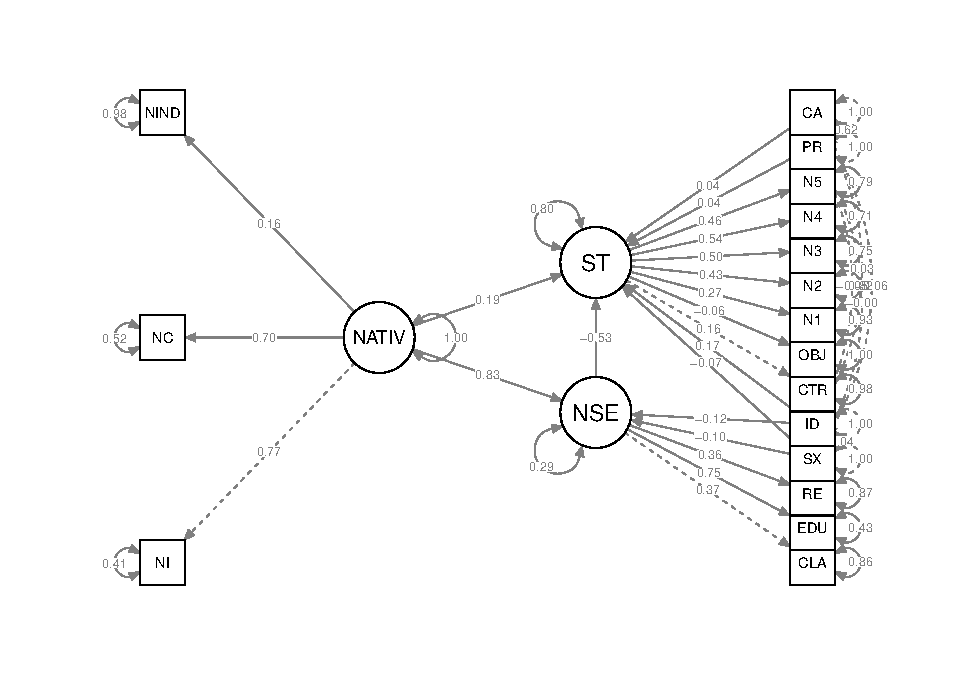
\includegraphics{trabalho_final_files/figure-latex/unnamed-chunk-2-1.pdf}

\normalsize
\onehalfspacing

Desta forma, obtivemos os seguintes resultados:

\scriptsize

\begin{Shaded}
\begin{Highlighting}[]
\CommentTok{\# Sumário com o resultado do Modelo 1}
\KeywordTok{summary}\NormalTok{(model.fit,}
\DataTypeTok{standardized =} \OtherTok{TRUE}\NormalTok{,}
\DataTypeTok{fit.measures =} \OtherTok{TRUE}\NormalTok{,}
\DataTypeTok{rsquare =} \OtherTok{TRUE}\NormalTok{)}
\end{Highlighting}
\end{Shaded}

\begin{verbatim}
## lavaan 0.6-7 ended normally after 132 iterations
## 
##   Estimator                                         ML
##   Optimization method                           NLMINB
##   Number of free parameters                         35
##                                                       
##                                                   Used       Total
##   Number of observations                           653        1500
##                                                                   
## Model Test User Model:
##                                                       
##   Test statistic                               323.299
##   Degrees of freedom                               108
##   P-value (Chi-square)                           0.000
## 
## Model Test Baseline Model:
## 
##   Test statistic                              1165.473
##   Degrees of freedom                               130
##   P-value                                        0.000
## 
## User Model versus Baseline Model:
## 
##   Comparative Fit Index (CFI)                    0.792
##   Tucker-Lewis Index (TLI)                       0.750
## 
## Loglikelihood and Information Criteria:
## 
##   Loglikelihood user model (H0)             -14478.803
##   Loglikelihood unrestricted model (H1)     -14317.153
##                                                       
##   Akaike (AIC)                               29027.606
##   Bayesian (BIC)                             29184.461
##   Sample-size adjusted Bayesian (BIC)        29073.336
## 
## Root Mean Square Error of Approximation:
## 
##   RMSEA                                          0.055
##   90 Percent confidence interval - lower         0.048
##   90 Percent confidence interval - upper         0.062
##   P-value RMSEA <= 0.05                          0.103
## 
## Standardized Root Mean Square Residual:
## 
##   SRMR                                           0.052
## 
## Parameter Estimates:
## 
##   Standard errors                             Standard
##   Information                                 Expected
##   Information saturated (h1) model          Structured
## 
## Latent Variables:
##                    Estimate  Std.Err  z-value  P(>|z|)   Std.lv  Std.all
##   NSE =~                                                                
##     CLA               1.000                               0.304    0.370
##     EDU               6.008    0.799    7.516    0.000    1.826    0.753
##     RE                2.487    0.416    5.982    0.000    0.756    0.361
##   NATIV =~                                                              
##     NI                1.000                               2.420    0.768
##     NC                0.873    0.068   12.764    0.000    2.113    0.696
##     NIND              0.192    0.056    3.449    0.001    0.464    0.156
##   ST =~                                                                 
##     CTR               1.000                               0.072    0.156
##     OBJ              -0.881    0.801   -1.100    0.271   -0.064   -0.059
##     N1                3.885    1.448    2.683    0.007    0.281    0.266
##     N2                6.913    2.365    2.923    0.003    0.500    0.428
##     N3                7.065    2.383    2.964    0.003    0.511    0.497
##     N4                7.003    2.351    2.979    0.003    0.506    0.539
##     N5                7.101    2.414    2.942    0.003    0.514    0.456
## 
## Regressions:
##                    Estimate  Std.Err  z-value  P(>|z|)   Std.lv  Std.all
##   NSE ~                                                                 
##     NATIV             0.104    0.015    7.036    0.000    0.826    0.826
##     SX               -0.062    0.026   -2.367    0.018   -0.203   -0.102
##     ID               -0.003    0.001   -2.786    0.005   -0.010   -0.122
##   ST ~                                                                  
##     SX               -0.011    0.009   -1.182    0.237   -0.146   -0.073
##     ID                0.001    0.000    2.083    0.037    0.013    0.165
##     NATIV             0.006    0.007    0.849    0.396    0.193    0.193
##     NSE              -0.127    0.069   -1.841    0.066   -0.532   -0.532
##     PR                0.007    0.012    0.596    0.551    0.097    0.039
##     CA                0.006    0.010    0.615    0.539    0.082    0.040
## 
## Variances:
##                    Estimate  Std.Err  z-value  P(>|z|)   Std.lv  Std.all
##    .CLA               0.584    0.034   17.013    0.000    0.584    0.863
##    .EDU               2.540    0.347    7.313    0.000    2.540    0.432
##    .RE                3.810    0.223   17.069    0.000    3.810    0.870
##    .NI                4.078    0.455    8.962    0.000    4.078    0.410
##    .NC                4.754    0.401   11.866    0.000    4.754    0.516
##    .NIND              8.676    0.484   17.927    0.000    8.676    0.976
##    .CTR               0.209    0.012   17.765    0.000    0.209    0.976
##    .OBJ               1.143    0.063   18.026    0.000    1.143    0.996
##    .N1                1.040    0.061   17.143    0.000    1.040    0.929
##    .N2                1.111    0.073   15.284    0.000    1.111    0.816
##    .N3                0.794    0.057   13.967    0.000    0.794    0.753
##    .N4                0.627    0.048   12.963    0.000    0.627    0.710
##    .N5                1.005    0.068   14.810    0.000    1.005    0.792
##    .NSE               0.027    0.010    2.791    0.005    0.292    0.292
##     NATIV             5.858    0.638    9.176    0.000    1.000    1.000
##    .ST                0.004    0.003    1.539    0.124    0.802    0.802
## 
## R-Square:
##                    Estimate
##     CLA               0.137
##     EDU               0.568
##     RE                0.130
##     NI                0.590
##     NC                0.484
##     NIND              0.024
##     CTR               0.024
##     OBJ               0.004
##     N1                0.071
##     N2                0.184
##     N3                0.247
##     N4                0.290
##     N5                0.208
##     NSE               0.708
##     ST                0.198
\end{verbatim}

\normalsize
\onehalfspacing

Antes de analisarmos a qualidade do modelo, faz-se necessário, portanto,
observar que, no construto, apenas a relação entre a variável latente de
significados do trabalho e a variável observável relativa aos resultados
esperados/valorizados no trabalho, representada pela sigla OBJ, não foi
estatisticamente significativa a um nível de 95\% de confiança uma vez
que \(P(>|z|) = 0.271\). Isto, portanto, significa dizer que, embora
tenha sido indicado pela literatura que esta variável seria importante
para a construção dos significados do trabalho, ela não foi
estatisticamente significativa no banco de dados analisado. Seriam
necessárias pesquisas com um maior contingente de observações para
analisar a relação entre a variável OBJ e o constructo ST.

Já na parte dos resultados referente às regressões, observamos que as
seguintes variáveis não apresentam coeficientes estatisticamente
significativos em relação à variável dependentes significados do
trabalho (ST): sexo (SX), natureza da atividade laboral (NATIV),
variável indicadora para protestantes (PR) e também a variável
indicadora para católicos (CA).

Posto isto, para analisarmos a qualidade geral do modelo, é importante
observamos as seguintes medidas: qui-quadrado, Standardized Root Mean
Square Residual (SRMSR), Root Mean Square Residual (RSMEA), Comparative
Fit Index (CFI) e o Tucker-Lewis Index (TLI).

Em relação à primeira medida, qui-quadrado, tem-se que ele consistiria,
segundo Pereira (\protect\hyperlink{ref-pereira2013modelagem}{2013}),
``em um teste de ajustamento da função de discrepância minimizada
durante o ajustamento do modelo'', cujas hipóteses nula e alternativa
correspondem, respectivamente, à ideia de que a matriz de covariância
populacional é igual ou diferente daquela estimada pelo modelo. De
acordo com o sumário dos resultados do Modelo 1, anteriormente exposto,
seu valor foi de \(323.299\), a \(108\) graus de liberdade. Além disto,
é importante observar que ele foi significativo a um nível de 99\% de
confiança (\(p-valor < 0.001\)), ou seja, aceitou a hipótese
alternativa.

Já no que se refere à segunda medida, SRMSR, cabe dizer que Pereira
(\protect\hyperlink{ref-pereira2013modelagem}{2013}, p. 25) a define
como sendo ``a raiz quadrada da matriz dos erros dividida pelos graus de
liberdade, assumindo que o modelo ajustado é o correto''. Ainda segundo
esta autora, tal medida deve ser interpretada como inversamente
proporcional à qualidade do ajuste, sendo que este será considerado bom
quando seu valor for igual ou menor que \(0.05\) (PEREIRA,
\protect\hyperlink{ref-pereira2013modelagem}{2013}). A partir da leitura
do sumário dos resultados do Modelo 1, observa-se que seu valor foi de
\(0.052\), ou seja, seu ajuste está um pouco acima do desejado, sendo
necessários ajustes para melhorar o SRMSR.

A RSMEA, por sua vez, estaria relacionada ao erro de aproximação na
população (PEREIRA, \protect\hyperlink{ref-pereira2013modelagem}{2013}).
De forma semelhante à SRMSR, para que indique um bom ajuste, portanto, é
necessário que apresente um valor inferior a \(0.05\). No entanto, como
fora indicado pelo sumário de resultados do modelo 1, seu ajuste é
apenas razoável, à medida em que obtivera o valor \(0.055\) para esta
medida.

Embora sua RSMEA, aponte para a razoabilidade de seu ajuste, as medidas
CFI e TLI apontam para sua má qualidade. Se, por um lado, a CFI seria a
razão entre o ajuste do modelo em questão e o pior modelo possível, por
outro, o TLI corresponderia a uma escala de qualidade do ajuste,
variando de 0 a 1. Para o Modelo 1, estas medidas obtiveram,
respectivamente, os valores \(0.792\) e \(0.750\), reforçando a ideia de
que seu ajuste pode ser melhorado.

Em busca de seu aprimoramento, nós utilizamos o comando
modificationindices, cuja principal função é indicar quais melhorias
podem ser implementadas para aumentar o ajuste do modelo. Por meio dele,
obtivemos os seguintes resultados:

\scriptsize

\begin{Shaded}
\begin{Highlighting}[]
\KeywordTok{modificationindices}\NormalTok{(model.fit, }\DataTypeTok{sort =} \OtherTok{TRUE}\NormalTok{, }\DataTypeTok{maximum.number =} \DecValTok{6}\NormalTok{)}
\end{Highlighting}
\end{Shaded}

\begin{verbatim}
##       lhs op rhs     mi    epc sepc.lv sepc.all sepc.nox
## 76    CLA ~~  RE 92.320  0.599   0.599    0.402    0.402
## 116    NI ~~  N5 16.392 -0.428  -0.428   -0.211   -0.211
## 67  NATIV =~  N4 15.686  0.076   0.185    0.197    0.197
## 57    NSE =~  N4 13.319  0.624   0.190    0.202    0.202
## 58    NSE =~  N5 12.343 -0.696  -0.212   -0.188   -0.188
## 97    EDU ~~  N5 10.387 -0.278  -0.278   -0.174   -0.174
\end{verbatim}

\normalsize
\onehalfspacing

Como é possível observar, o comando, anteriormente mencionado, apontou
para a existência de covariância entre os seguintes pares de variáveis:
classe (CLA) e rendimento (RE); nível de atividades manuais a
intelectuais (NI) e ``o trabalho sempre deve ser posto em primeiro
lugar'' (N5); educação (EDU) e a variável N5. Além disto, seu resultado
também indicou a possibilidade de inclusão no constructo da natureza da
atividade laboral (NATIV) a variável ``trabalhar é uma obrigação para
com a sociedade'' (N4), e no constructo do nível socioeconômico (NSE) as
variáveis N4 e N5.

Após uma série de discussões entre os membros do nosso grupo, optamos
pela incorporação das relações de covariância existente entre os pares
classe (CLA) e rendimento (RE); nível de atividades manuais a
intelectuais (NI) e ``o trabalho sempre deve ser posto em primeiro
lugar'' (N5); educação (EDU) e a variável N5. Nesta mesma fase do
trabalho, também optamos por incluir a relação entre as variáveis entre
a natureza da atividade laboral (NATIV) e ``trabalhar é uma obrigação
para com a sociedade'' (N4). Tal esforço seria importante à medida em
que nos possibilitaria remediar o efeito de relações espúrias existentes
entre as variáveis latentes e observáveis incluídas em nossos modelos.

\hypertarget{modelo-2}{%
\section{Modelo 2}\label{modelo-2}}

\scriptsize
\singlespacing

\begin{Shaded}
\begin{Highlighting}[]
\CommentTok{\# Modelo 2 {-} MEE}
\NormalTok{model\_}\DecValTok{2}\NormalTok{ \textless{}{-}}\StringTok{ "}
\StringTok{NSE =\textasciitilde{} CLA + EDU + RE}
\StringTok{NATIV =\textasciitilde{} NI + NC + NIND}
\StringTok{NSE \textasciitilde{} NATIV + SX + ID}
\StringTok{ST =\textasciitilde{} CTR + OBJ + N1 + N2 + N3 + N4 + N5}
\StringTok{ST \textasciitilde{} SX + ID + NATIV + NSE + PR + CA}
\StringTok{CLA \textasciitilde{}\textasciitilde{} RE}
\StringTok{NATIV =\textasciitilde{} N4}
\StringTok{NI \textasciitilde{}\textasciitilde{} N5}
\StringTok{EDU \textasciitilde{}\textasciitilde{} N5}
\StringTok{"}

\NormalTok{model\_}\FloatTok{2.}\NormalTok{fit \textless{}{-}}\StringTok{ }\KeywordTok{cfa}\NormalTok{(model\_}\DecValTok{2}\NormalTok{, }\DataTypeTok{data =}\NormalTok{ df\_}\DecValTok{2}\NormalTok{)}

\KeywordTok{semPaths}\NormalTok{(model\_}\FloatTok{2.}\NormalTok{fit,}
         \DataTypeTok{whatLabels =} \StringTok{"std"}\NormalTok{,}
         \DataTypeTok{layout =} \StringTok{"tree"}\NormalTok{,}
         \DataTypeTok{residuals =} \OtherTok{TRUE}\NormalTok{,}
         \DataTypeTok{rotation =} \DecValTok{2}\NormalTok{,}
         \DataTypeTok{nCharNodes =} \DecValTok{0}\NormalTok{)}
\end{Highlighting}
\end{Shaded}

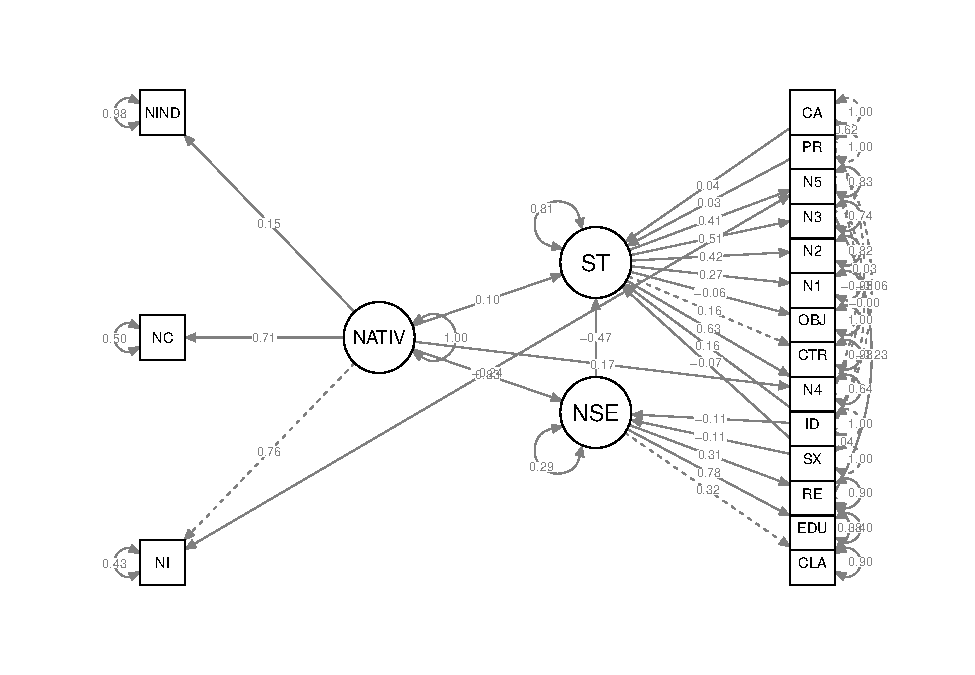
\includegraphics{trabalho_final_files/figure-latex/unnamed-chunk-5-1.pdf}

\normalsize
\onehalfspacing

\hypertarget{comparauxe7uxe3o-dos-modelos}{%
\section{Comparação dos modelos}\label{comparauxe7uxe3o-dos-modelos}}

\hypertarget{modelo-1}{%
\subsection{Modelo 1}\label{modelo-1}}

\scriptsize
\singlespacing

\begin{Shaded}
\begin{Highlighting}[]
\KeywordTok{fitmeasures}\NormalTok{(model.fit, }\KeywordTok{c}\NormalTok{(}\StringTok{"cfi"}\NormalTok{, }\StringTok{"tli"}\NormalTok{, }\StringTok{"rmsea"}\NormalTok{))}
\end{Highlighting}
\end{Shaded}

\begin{verbatim}
##   cfi   tli rmsea 
## 0.792 0.750 0.055
\end{verbatim}

\normalsize
\onehalfspacing

\hypertarget{modelo-2-1}{%
\subsection{Modelo 2}\label{modelo-2-1}}

\scriptsize
\singlespacing

\begin{Shaded}
\begin{Highlighting}[]
\KeywordTok{fitmeasures}\NormalTok{(model\_}\FloatTok{2.}\NormalTok{fit, }\KeywordTok{c}\NormalTok{(}\StringTok{"cfi"}\NormalTok{, }\StringTok{"tli"}\NormalTok{, }\StringTok{"rmsea"}\NormalTok{))}
\end{Highlighting}
\end{Shaded}

\begin{verbatim}
##   cfi   tli rmsea 
## 0.923 0.904 0.034
\end{verbatim}

\begin{Shaded}
\begin{Highlighting}[]
\CommentTok{\# Sumário com o resultado do Modelo 2}
\KeywordTok{summary}\NormalTok{(model\_}\FloatTok{2.}\NormalTok{fit,}
\DataTypeTok{standardized =} \OtherTok{TRUE}\NormalTok{,}
\DataTypeTok{fit.measures =} \OtherTok{TRUE}\NormalTok{,}
\DataTypeTok{rsquare =} \OtherTok{TRUE}\NormalTok{)}
\end{Highlighting}
\end{Shaded}

\begin{verbatim}
## lavaan 0.6-7 ended normally after 139 iterations
## 
##   Estimator                                         ML
##   Optimization method                           NLMINB
##   Number of free parameters                         39
##                                                       
##                                                   Used       Total
##   Number of observations                           653        1500
##                                                                   
## Model Test User Model:
##                                                       
##   Test statistic                               183.645
##   Degrees of freedom                               104
##   P-value (Chi-square)                           0.000
## 
## Model Test Baseline Model:
## 
##   Test statistic                              1165.473
##   Degrees of freedom                               130
##   P-value                                        0.000
## 
## User Model versus Baseline Model:
## 
##   Comparative Fit Index (CFI)                    0.923
##   Tucker-Lewis Index (TLI)                       0.904
## 
## Loglikelihood and Information Criteria:
## 
##   Loglikelihood user model (H0)             -14408.976
##   Loglikelihood unrestricted model (H1)     -14317.153
##                                                       
##   Akaike (AIC)                               28895.952
##   Bayesian (BIC)                             29070.733
##   Sample-size adjusted Bayesian (BIC)        28946.909
## 
## Root Mean Square Error of Approximation:
## 
##   RMSEA                                          0.034
##   90 Percent confidence interval - lower         0.026
##   90 Percent confidence interval - upper         0.042
##   P-value RMSEA <= 0.05                          1.000
## 
## Standardized Root Mean Square Residual:
## 
##   SRMR                                           0.040
## 
## Parameter Estimates:
## 
##   Standard errors                             Standard
##   Information                                 Expected
##   Information saturated (h1) model          Structured
## 
## Latent Variables:
##                    Estimate  Std.Err  z-value  P(>|z|)   Std.lv  Std.all
##   NSE =~                                                                
##     CLA               1.000                               0.264    0.320
##     EDU               7.166    1.136    6.308    0.000    1.888    0.778
##     RE                2.468    0.379    6.512    0.000    0.650    0.311
##   NATIV =~                                                              
##     NI                1.000                               2.393    0.758
##     NC                0.898    0.069   13.084    0.000    2.150    0.708
##     NIND              0.184    0.056    3.299    0.001    0.441    0.148
##   ST =~                                                                 
##     CTR               1.000                               0.073    0.157
##     OBJ              -0.910    0.791   -1.151    0.250   -0.066   -0.062
##     N1                3.924    1.434    2.737    0.006    0.285    0.270
##     N2                6.747    2.274    2.968    0.003    0.490    0.420
##     N3                7.143    2.365    3.020    0.003    0.519    0.505
##     N4                8.086    2.682    3.015    0.003    0.588    0.625
##     N5                6.407    2.161    2.965    0.003    0.466    0.413
##   NATIV =~                                                              
##     N4                0.065    0.021    3.108    0.002    0.156    0.166
## 
## Regressions:
##                    Estimate  Std.Err  z-value  P(>|z|)   Std.lv  Std.all
##   NSE ~                                                                 
##     NATIV             0.091    0.015    6.024    0.000    0.829    0.829
##     SX               -0.059    0.023   -2.548    0.011   -0.223   -0.111
##     ID               -0.002    0.001   -2.554    0.011   -0.009   -0.112
##   ST ~                                                                  
##     SX               -0.010    0.009   -1.081    0.280   -0.132   -0.066
##     ID                0.001    0.000    2.069    0.039    0.012    0.157
##     NATIV             0.003    0.007    0.417    0.677    0.102    0.102
##     NSE              -0.129    0.080   -1.610    0.107   -0.469   -0.469
##     PR                0.006    0.011    0.551    0.582    0.086    0.034
##     CA                0.005    0.009    0.588    0.557    0.075    0.037
## 
## Covariances:
##                    Estimate  Std.Err  z-value  P(>|z|)   Std.lv  Std.all
##  .CLA ~~                                                                
##    .RE                0.584    0.068    8.561    0.000    0.584    0.376
##  .NI ~~                                                                 
##    .N5               -0.510    0.113   -4.495    0.000   -0.510   -0.241
##  .EDU ~~                                                                
##    .N5               -0.357    0.091   -3.910    0.000   -0.357   -0.228
## 
## Variances:
##                    Estimate  Std.Err  z-value  P(>|z|)   Std.lv  Std.all
##    .CLA               0.607    0.035   17.317    0.000    0.607    0.897
##    .EDU               2.330    0.462    5.049    0.000    2.330    0.395
##    .RE                3.959    0.228   17.366    0.000    3.959    0.904
##    .NI                4.252    0.443    9.596    0.000    4.252    0.426
##    .NC                4.599    0.394   11.663    0.000    4.599    0.499
##    .NIND              8.697    0.485   17.947    0.000    8.697    0.978
##    .CTR               0.209    0.012   17.779    0.000    0.209    0.975
##    .OBJ               1.143    0.063   18.025    0.000    1.143    0.996
##    .N1                1.038    0.060   17.160    0.000    1.038    0.927
##    .N2                1.121    0.072   15.514    0.000    1.121    0.823
##    .N3                0.786    0.057   13.871    0.000    0.786    0.745
##    .N4                0.566    0.053   10.642    0.000    0.566    0.641
##    .N5                1.052    0.067   15.621    0.000    1.052    0.829
##    .NSE               0.020    0.008    2.366    0.018    0.287    0.287
##     NATIV             5.728    0.621    9.222    0.000    1.000    1.000
##    .ST                0.004    0.003    1.564    0.118    0.810    0.810
## 
## R-Square:
##                    Estimate
##     CLA               0.103
##     EDU               0.605
##     RE                0.096
##     NI                0.574
##     NC                0.501
##     NIND              0.022
##     CTR               0.025
##     OBJ               0.004
##     N1                0.073
##     N2                0.177
##     N3                0.255
##     N4                0.359
##     N5                0.171
##     NSE               0.713
##     ST                0.190
\end{verbatim}

\normalsize
\onehalfspacing

Ao compararmos os resultados obtidos pelo Modelo 2 com aqueles obtidos
pelo Modelo 1, observamos que todas as medidas de ajuste melhoraram. Em
relação ao qui-quadrado, notamos que, no Modelo 2, seu valor foi
\(183.645\), a \(104\) graus de liberdade, mantendo-se estatisticamente
significativo ao nível de \(99\%\) de confiança (\(p-valor < 0,001\)),
ou seja, também aceitou a hipótese alternativa. No que diz respeito à
medida SRMR, observamos que seu valor obtido, no Modelo 2, foi
\(0.040\), indicando, portanto, que seu ajuste é melhor do que aquele
que fora apresentado pelo Modelo 1. Tal tendência de melhoria no ajuste,
apenas foi reforçada pelas medidas RSMEA, CFI e TLI, cujos novos valores
foram: \(0.034\); \(0.934\) e \(0.904\), nesta sequência.

\hypertarget{modelo-3}{%
\section{Modelo 3}\label{modelo-3}}

Embora o Modelo 2 tenha apresentado grandes avanços na qualidade do
ajuste, nosso grupo decidiu por rodar o Modelo 3. Tendo em vista que, no
construto ST, a variável OBJ se manteve estatisticamente não
significativa, assim como as variáveis sexo (SX), natureza da atividade
laboral (NATIV), variável indicadora para católicos (CA) e protestantes
(PR) nas regressões, nós optamos pela exclusão das mesmas em nossa
terceira tentativa. Para tanto, compilamos os seguintes comandos:

\scriptsize
\singlespacing

\begin{Shaded}
\begin{Highlighting}[]
\CommentTok{\# Modelo 3 {-} MEE}
\NormalTok{model\_}\DecValTok{3}\NormalTok{ \textless{}{-}}\StringTok{ "}
\StringTok{NSE =\textasciitilde{} CLA + EDU + RE}
\StringTok{NATIV =\textasciitilde{} NI + NC + NIND}
\StringTok{NSE \textasciitilde{} NATIV + SX + ID}
\StringTok{ST =\textasciitilde{} CTR + N1 + N2 + N3 + N4 + N5}
\StringTok{ST \textasciitilde{} ID + NSE}
\StringTok{CLA \textasciitilde{}\textasciitilde{}  RE}
\StringTok{NATIV   =\textasciitilde{}  N4}
\StringTok{NI  \textasciitilde{}\textasciitilde{}  N5}
\StringTok{EDU \textasciitilde{}\textasciitilde{}  N5}
\StringTok{"}

\NormalTok{model\_}\FloatTok{3.}\NormalTok{fit \textless{}{-}}\StringTok{ }\KeywordTok{cfa}\NormalTok{(model\_}\DecValTok{3}\NormalTok{, }\DataTypeTok{data =}\NormalTok{ df\_}\DecValTok{2}\NormalTok{)}

\KeywordTok{semPaths}\NormalTok{(model\_}\FloatTok{3.}\NormalTok{fit,}
         \DataTypeTok{whatLabels =} \StringTok{"std"}\NormalTok{,}
         \DataTypeTok{layout =} \StringTok{"tree"}\NormalTok{,}
         \DataTypeTok{residuals =} \OtherTok{TRUE}\NormalTok{,}
         \DataTypeTok{rotation =} \DecValTok{2}\NormalTok{,}
         \DataTypeTok{nCharNodes =} \DecValTok{0}\NormalTok{)}
\end{Highlighting}
\end{Shaded}

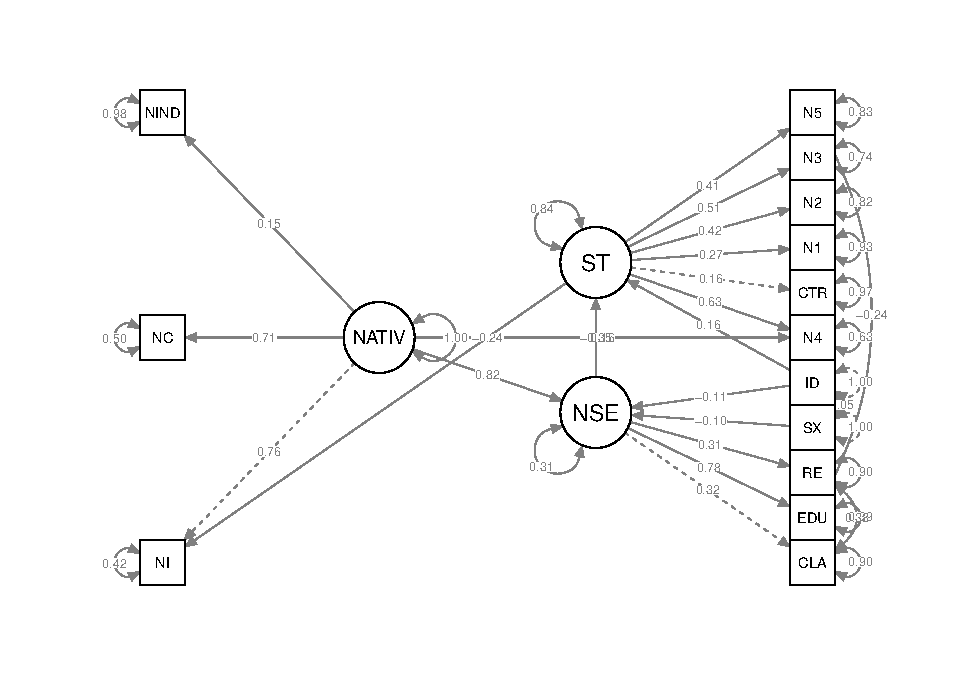
\includegraphics{trabalho_final_files/figure-latex/unnamed-chunk-9-1.pdf}

\normalsize
\onehalfspacing

Tais comandos nos possibilitaram a obtenção dos seguintes resultados:

\scriptsize
\singlespacing

\hypertarget{comparauxe7uxe3o-dos-modelos-1}{%
\subsection{Comparação dos
Modelos}\label{comparauxe7uxe3o-dos-modelos-1}}

\hypertarget{modelo-1-1}{%
\subsubsection{Modelo 1}\label{modelo-1-1}}

\begin{Shaded}
\begin{Highlighting}[]
\KeywordTok{fitmeasures}\NormalTok{(model.fit, }\KeywordTok{c}\NormalTok{(}\StringTok{"cfi"}\NormalTok{, }\StringTok{"tli"}\NormalTok{, }\StringTok{"rmsea"}\NormalTok{))}
\end{Highlighting}
\end{Shaded}

\begin{verbatim}
##   cfi   tli rmsea 
## 0.792 0.750 0.055
\end{verbatim}

\hypertarget{modelo-2-2}{%
\subsubsection{Modelo 2}\label{modelo-2-2}}

\begin{Shaded}
\begin{Highlighting}[]
\KeywordTok{fitmeasures}\NormalTok{(model\_}\FloatTok{2.}\NormalTok{fit, }\KeywordTok{c}\NormalTok{(}\StringTok{"cfi"}\NormalTok{, }\StringTok{"tli"}\NormalTok{, }\StringTok{"rmsea"}\NormalTok{))}
\end{Highlighting}
\end{Shaded}

\begin{verbatim}
##   cfi   tli rmsea 
## 0.923 0.904 0.034
\end{verbatim}

\hypertarget{modelo-3-1}{%
\subsubsection{Modelo 3}\label{modelo-3-1}}

\begin{Shaded}
\begin{Highlighting}[]
\KeywordTok{fitmeasures}\NormalTok{(model\_}\FloatTok{3.}\NormalTok{fit, }\KeywordTok{c}\NormalTok{(}\StringTok{"cfi"}\NormalTok{, }\StringTok{"tli"}\NormalTok{, }\StringTok{"rmsea"}\NormalTok{))}
\end{Highlighting}
\end{Shaded}

\begin{verbatim}
##   cfi   tli rmsea 
## 0.944 0.928 0.035
\end{verbatim}

\begin{Shaded}
\begin{Highlighting}[]
\CommentTok{\# Sumário com o resultado do Modelo 3}
\KeywordTok{summary}\NormalTok{(model\_}\FloatTok{3.}\NormalTok{fit,}
\DataTypeTok{standardized =} \OtherTok{TRUE}\NormalTok{,}
\DataTypeTok{fit.measures =} \OtherTok{TRUE}\NormalTok{,}
\DataTypeTok{rsquare =} \OtherTok{TRUE}\NormalTok{)}
\end{Highlighting}
\end{Shaded}

\begin{verbatim}
## lavaan 0.6-7 ended normally after 122 iterations
## 
##   Estimator                                         ML
##   Optimization method                           NLMINB
##   Number of free parameters                         33
##                                                       
##                                                   Used       Total
##   Number of observations                           656        1500
##                                                                   
## Model Test User Model:
##                                                       
##   Test statistic                               125.628
##   Degrees of freedom                                69
##   P-value (Chi-square)                           0.000
## 
## Model Test Baseline Model:
## 
##   Test statistic                              1110.226
##   Degrees of freedom                                90
##   P-value                                        0.000
## 
## User Model versus Baseline Model:
## 
##   Comparative Fit Index (CFI)                    0.944
##   Tucker-Lewis Index (TLI)                       0.928
## 
## Loglikelihood and Information Criteria:
## 
##   Loglikelihood user model (H0)             -13500.974
##   Loglikelihood unrestricted model (H1)     -13438.160
##                                                       
##   Akaike (AIC)                               27067.948
##   Bayesian (BIC)                             27215.991
##   Sample-size adjusted Bayesian (BIC)        27111.216
## 
## Root Mean Square Error of Approximation:
## 
##   RMSEA                                          0.035
##   90 Percent confidence interval - lower         0.025
##   90 Percent confidence interval - upper         0.045
##   P-value RMSEA <= 0.05                          0.994
## 
## Standardized Root Mean Square Residual:
## 
##   SRMR                                           0.040
## 
## Parameter Estimates:
## 
##   Standard errors                             Standard
##   Information                                 Expected
##   Information saturated (h1) model          Structured
## 
## Latent Variables:
##                    Estimate  Std.Err  z-value  P(>|z|)   Std.lv  Std.all
##   NSE =~                                                                
##     CLA               1.000                               0.266    0.323
##     EDU               7.151    1.102    6.489    0.000    1.902    0.782
##     RE                2.478    0.375    6.610    0.000    0.659    0.314
##   NATIV =~                                                              
##     NI                1.000                               2.397    0.760
##     NC                0.897    0.069   13.052    0.000    2.150    0.708
##     NIND              0.188    0.056    3.365    0.001    0.450    0.151
##   ST =~                                                                 
##     CTR               1.000                               0.073    0.158
##     N1                3.834    1.392    2.754    0.006    0.281    0.266
##     N2                6.663    2.221    3.000    0.003    0.489    0.419
##     N3                7.082    2.318    3.055    0.002    0.520    0.506
##     N4                8.099    2.653    3.053    0.002    0.594    0.632
##     N5                6.376    2.125    3.000    0.003    0.468    0.415
##   NATIV =~                                                              
##     N4                0.063    0.020    3.060    0.002    0.150    0.160
## 
## Regressions:
##                    Estimate  Std.Err  z-value  P(>|z|)   Std.lv  Std.all
##   NSE ~                                                                 
##     NATIV             0.091    0.015    6.210    0.000    0.817    0.817
##     SX               -0.054    0.023   -2.401    0.016   -0.204   -0.102
##     ID               -0.002    0.001   -2.447    0.014   -0.008   -0.105
##   ST ~                                                                  
##     ID                0.001    0.000    2.303    0.021    0.013    0.163
##     NSE              -0.098    0.037   -2.615    0.009   -0.354   -0.354
## 
## Covariances:
##                    Estimate  Std.Err  z-value  P(>|z|)   Std.lv  Std.all
##  .CLA ~~                                                                
##    .RE                0.589    0.068    8.620    0.000    0.589    0.379
##  .NI ~~                                                                 
##    .N5               -0.508    0.112   -4.537    0.000   -0.508   -0.242
##  .EDU ~~                                                                
##    .N5               -0.374    0.091   -4.122    0.000   -0.374   -0.241
## 
## Variances:
##                    Estimate  Std.Err  z-value  P(>|z|)   Std.lv  Std.all
##    .CLA               0.607    0.035   17.330    0.000    0.607    0.896
##    .EDU               2.293    0.409    5.610    0.000    2.293    0.388
##    .RE                3.969    0.228   17.378    0.000    3.969    0.901
##    .NI                4.206    0.444    9.479    0.000    4.206    0.423
##    .NC                4.595    0.395   11.643    0.000    4.595    0.499
##    .NIND              8.715    0.485   17.984    0.000    8.715    0.977
##    .CTR               0.209    0.012   17.815    0.000    0.209    0.975
##    .N1                1.038    0.060   17.227    0.000    1.038    0.929
##    .N2                1.120    0.072   15.567    0.000    1.120    0.824
##    .N3                0.783    0.056   13.875    0.000    0.783    0.744
##    .N4                0.558    0.053   10.483    0.000    0.558    0.633
##    .N5                1.052    0.067   15.653    0.000    1.052    0.828
##    .NSE               0.022    0.008    2.715    0.007    0.309    0.309
##     NATIV             5.746    0.621    9.249    0.000    1.000    1.000
##    .ST                0.004    0.003    1.588    0.112    0.836    0.836
## 
## R-Square:
##                    Estimate
##     CLA               0.104
##     EDU               0.612
##     RE                0.099
##     NI                0.577
##     NC                0.501
##     NIND              0.023
##     CTR               0.025
##     N1                0.071
##     N2                0.176
##     N3                0.256
##     N4                0.367
##     N5                0.172
##     NSE               0.691
##     ST                0.164
\end{verbatim}

\normalsize
\onehalfspacing

Sendo assim, quando comparamos os resultados obtidos pelo Modelo 3 com
aqueles obtidos pelos modelos anteriores, observamos que as medidas de
ajuste melhoraram, exceto SRMSR e RMSEA, cujos valores permaneceram,
aproximadamente, iguais àqueles que haviam apresentado no segundo
modelo. Ao analisarmos o qui-quadrado, observamos que, no Modelo 3, seu
valor foi de \(125.628\), a \(69\) graus de liberdade, mantendo-se
estatisticamente significativo ao nível de \(99\%\) de confiança
(\(p-valor < 0.001\)), aceitando também a hipótese alternativa. Já em
relação às medidas CFI e TLI, observamos que seus novos valores foram,
respectivamente, \(0.944\) e \(0.928\).

A partir dos resultados, aqui, analisados, considerando os objetivos
deste trabalho, concluímos afirmando que o Modelo 3 seria o modelo que
nós escolheríamos, à medida em que é aquele que apresentou as melhores
medidas de ajuste.

\hypertarget{considerauxe7uxf5es-finais}{%
\section{Considerações Finais}\label{considerauxe7uxf5es-finais}}

Este estudo realizou a estimação dos dados do World Values Survey (WVS)
para o Brasil por meio do software R. Vale mencionar que a base de dados
WVS disponibilizava a medida das seguintes dimensões: 1) Centralidade
absoluta do trabalho; 2) Normas sociais relativas ao trabalho como uma
obrigação e 3) Resultados esperados/valorizados no trabalho. Essas três
dimensões compõem o construto latente dos Significados do Trabalho.

Para tanto foram analisadas as variáveis elencadas na pesquisa WVS por
meio do Modelo de Equações Estruturais (MEE). O uso deste modelo é
justificado porque é uma técnica multivariada de caráter geral, que
combina a análise fatorial e análise de regressão. Além do que, modelos
de equações estruturais permitem que se trabalhe de forma simultânea a
estimação e mensuração, bem como a estimação de efeitos diretos e
indiretos. Destaca-se que estes modelos são considerados bastante
robustos e apresentam facilidade interpretativa (NEVES,
\protect\hyperlink{ref-neves2018modelo}{2018}).

Portanto, considerando que a proposta deste trabalho era de chegar a
opção que melhor se ajusta aos dados disponíveis na base de dados
disponibilizada, através do percurso metodológico e direcionamento do
modelo de equações estruturais, percebeu-se que o Modelo 3 seria o
modelo que apresentou as melhores medidas de ajuste. Corrobora para esta
afirmativa as observações acerca dos testes de qualidade de ajustes que
foram realizados.

\hypertarget{bibliografia}{%
\section*{Bibliografia}\label{bibliografia}}
\addcontentsline{toc}{section}{Bibliografia}

\hypertarget{refs}{}
\begin{cslreferences}
\leavevmode\hypertarget{ref-neves2018modelo}{}%
NEVES, J. A. B. Modelo de equações estruturais: uma introdução aplicada.
2018.

\leavevmode\hypertarget{ref-pereira2013modelagem}{}%
PEREIRA, S. DOS S. Modelagem de equações estruturais no software R.
2013.
\end{cslreferences}

\end{document}
